%%% fs-seim-stream - Stream processing concepts

\label {fs-stream}

In this section we define some preliminaries for distributed stream processing. It allows us to unify required terms and to introduce definitions, which are needed for the further statements.

Commonly, stream processing system is a shared-nothing distributed runtime that handles a potentially unbounded number of input events and processes them one-by-one, according to the procedures provided by a user. The main purpose of this kind of data processing systems is to provide low latency between event occurrence and its processing. Term {\it distributed} implies that user's procedures can have partitions on distinct computational units or shards. The following subsections detail the properties of such systems more precisely.  

\subsection{Data flow}
The basic data flow abstraction is a {\it stream}. The stream is an infinite sequence of events or data items. Each data item contains payload defined by a user. Besides, it can be assigned by meta-information. Usually, meta-information is used to define an order on data items. For instance, it can be represented as a UNIX timestamp in milliseconds with a trace of applied operations.

\subsection{Computation flow}
Commonly, the computational pipeline is defined in the form of {\it logical graph}. The vertices of the logical graph are operations, and edges are links between them. Logical graph defines only relations between operations, but it does not detail its physical deployment. The logical graph for the pipeline shown in the figure~\ref{break-order-dataflow} is presented in the figure~\ref{break-order-dataflow-logical}

\begin{figure}[htbp]
  \centering
  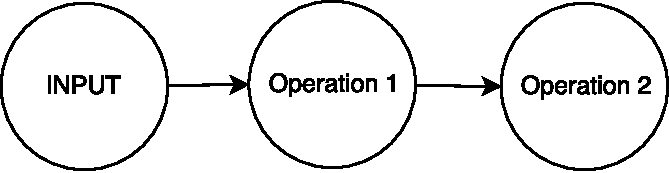
\includegraphics[width=0.38\textwidth]{pics/break_order_pipeline_logical}
  \caption{The logical graph}
  \label {break-order-dataflow-logical}
\end{figure}

\subsection{Operations}
There are two main types of streaming operations: {\it stateless} and {\it stateful}. Stateless operations do not need any knowledge about past inputs to correctly process current one. A simple illustration is a map operation that multiplies by 2 any input item's payload. On the other hand, stateful operations are able to keep some aggregations or summaries of received events. In such case, the output of operation depends not only on input but on its current state. As an example, an operation that reacts on each input item's payload with the sum of it and all previous payloads can be mentioned. 

\subsection{Physical deployment}
As it was mentioned above, each operation can be partitioned between multiple shards. Data items can be balanced between partitions by key extracted from item's payload for stateful operations or randomly for stateless. The schema of physical partitioning of operations is sometimes called {\it physical graph}. Regarding physical links between operations, in the most cases, it is supposed that they guarantee FIFO order.

\subsection{Guarantees}
Guarantees of stream processing declare the properties of data safety in case of system failures. There are three main types of such guarantees. {\it At most once} semantics states that each input event is processed once or not processed at all. {\it At least once} guarantees that each input item is processed, but possibly multiple times, that can lead to result duplication. {\it Exactly once} semantics guarantee that each input event is processed exactly one time.  
